\documentclass[tikz, border=20pt]{standalone}
\usepackage{amsmath, amssymb}
\usepackage{xcolor}
\usetikzlibrary{decorations.pathreplacing, positioning, calc}

\begin{document}
	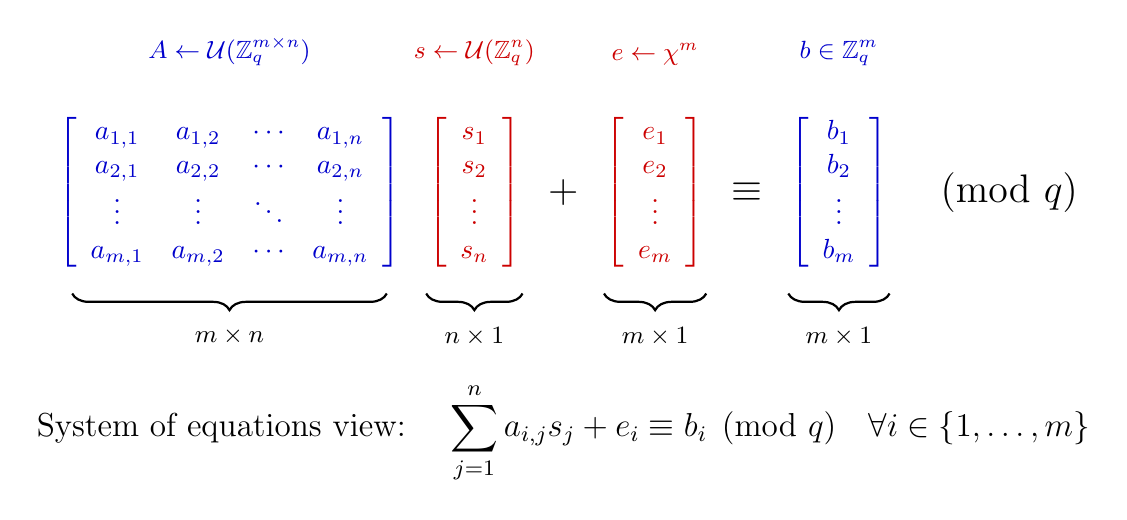
\begin{tikzpicture}[
		>=stealth,
		public/.style={text=blue!80!black},
		secret/.style={text=red!80!black}
		]
		
		% ==========================================
		% MATRIX A (Public)
		% ==========================================
		\node[public] (A) {
			$\left[
			\begin{array}{cccc}
				a_{1,1} & a_{1,2} & \cdots & a_{1,n} \\
				a_{2,1} & a_{2,2} & \cdots & a_{2,n} \\
				\vdots  & \vdots  & \ddots & \vdots  \\
				a_{m,1} & a_{m,2} & \cdots & a_{m,n}
			\end{array}
			\right]$
		};
		
		% ==========================================
		% VECTOR s (Secret)
		% ==========================================
		\node[secret, right=0.1cm of A] (s) {
			$\left[
			\begin{array}{c}
				s_1 \\ s_2 \\ \vdots \\ s_n
			\end{array}
			\right]$
		};
		
		% Plus Sign
		\node[right=0.1cm of s, font=\Large\bfseries] (plus) {$+$};
		
		% ==========================================
		% VECTOR e (Error / Secret)
		% ==========================================
		\node[secret, right=0.1cm of plus] (e) {
			$\left[
			\begin{array}{c}
				e_1 \\ e_2 \\ \vdots \\ e_m
			\end{array}
			\right]$
		};
		
		% Equals Sign
		\node[right=0.1cm of e, font=\Large\bfseries] (eq) {$\equiv$};
		
		% ==========================================
		% VECTOR b (Public Output)
		% ==========================================
		\node[public, right=0.1cm of eq] (b) {
			$\left[
			\begin{array}{c}
				b_1 \\ b_2 \\ \vdots \\ b_m
			\end{array}
			\right]$
		};
		
		% Modulo
		\node[right=0.2cm of b, font=\Large] (mod) {$\pmod q$};
		
		% ==========================================
		% DIMENSION BRACES
		% ==========================================
		\draw[decorate,decoration={brace,amplitude=6pt,mirror}, thick]
		([yshift=-0.2cm, xshift=0.3cm]A.south west) -- ([yshift=-0.2cm, xshift=-0.3cm]A.south east) 
		node[midway, below=0.3cm, font=\small] {$m \times n$};
		
		\draw[decorate,decoration={brace,amplitude=6pt,mirror}, thick]
		([yshift=-0.2cm, xshift=0.1cm]s.south west) -- ([yshift=-0.2cm, xshift=-0.1cm]s.south east) 
		node[midway, below=0.3cm, font=\small] {$n \times 1$};
		
		\draw[decorate,decoration={brace,amplitude=6pt,mirror}, thick]
		([yshift=-0.2cm, xshift=0.1cm]e.south west) -- ([yshift=-0.2cm, xshift=-0.1cm]e.south east) 
		node[midway, below=0.3cm, font=\small] {$m \times 1$};
		
		\draw[decorate,decoration={brace,amplitude=6pt,mirror}, thick]
		([yshift=-0.2cm, xshift=0.1cm]b.south west) -- ([yshift=-0.2cm, xshift=-0.1cm]b.south east) 
		node[midway, below=0.3cm, font=\small] {$m \times 1$};
		
		% ==========================================
		% DISTRIBUTION LABELS
		% ==========================================
		\node[above=0.4cm of A, public, font=\small] {$A \leftarrow \mathcal{U}(\mathbb{Z}_q^{m \times n})$};
		\node[above=0.4cm of s, secret, font=\small] {$s \leftarrow \mathcal{U}(\mathbb{Z}_q^n)$};
		\node[above=0.4cm of e, secret, font=\small] {$e \leftarrow \chi^m$};
		\node[above=0.4cm of b, public, font=\small] {$b \in \mathbb{Z}_q^m$};
		
		% ==========================================
		% LINEAR SYSTEM ANNOTATION
		% ==========================================
		\node[below=2cm of plus, font=\large] (system) {
			System of equations view: \hspace{0.2cm} 
			$\displaystyle \sum_{j=1}^{n} a_{i,j} s_j + e_i \equiv b_i \pmod q \quad \forall i \in \{1, \dots, m\}$
		};
		
	\end{tikzpicture}
\end{document}